\subsection{Dual Quaternion Skinning}

Da Linear Blend Skinning, wie wir gesehen haben ubiquit�r eingesetzt wird aber  oft zu Artefakten f�hrt, kann man laut \cite{kavan2008geometric} diesen Algorithmus leicht, durch Erweiterung des linearen Ansatz Dual Quaternionen mit einzubeziehen, optimieren und mit minimalen Aufwand aufwerten. 

\begin{figure}[t]
	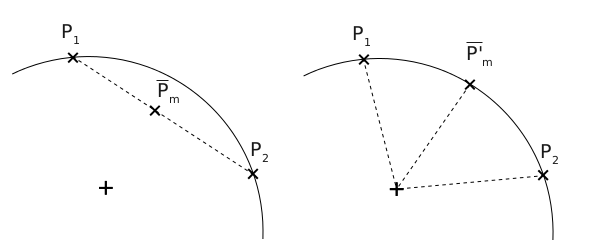
\includegraphics[width=7cm]{01_Skinning/pics/interpolation_angle.png}
	\caption[Vergleich im zweidimensionalen Raum]{ Darstellung im zweidimensionalen euklidischen Raum. Entnommen von \cite{kavan2008geometric}.}
	\label{weights_fig1}
\end{figure}

In Abbildung 9 ist eine vereinfachte Darstellung im zweidimensionalen euklidischen Raum. In Linear Blend Skinning vergleicht man essentiell die durchschnittliche Position wo ein Punkt liegen m�sste, was wie man links sieht unter Umst�nden zu Volumenverlust und damit zu Artefakten f�hrt. Vergleicht man hingegen wie rechts die durchschnittlichen Winkel, kann man Volumenverlust vermeiden.

Ein Weg dies zu erreichen ist von \cite{kavan2008geometric}, denn sie Dual Quaternion Linear Blending nennen. Ein Quaternion ist im Prinzip ein Vektor, mit einer Drehachse. Jede Dual-Zahl wird folgender weise dargestellt: $a + \varepsilon b$ wobei $\varepsilon^2 = 0$ ist. Ein Dual Quaternion kann also einfach als $\mathbf{\dot q} = \mathbf q_0 + \varepsilon \mathbf q_e$ bezeichnet. Wie in \cite{kavan2008geometric} bewiesen kann jede 4*4 Matrize, und damit jede Translation und Transformation, als Dual Quaternion dargestellt werden. Womit wir dann bei folgender Formal nach \cite{kavan2008geometric} landen: 

\begin{equation}
\label{formel}
$\mathbf{\dot q} =  \frac{\sum_{i=1}^n w_i \mathbf{\dot q}_i}{\| \sum_{i=1}^n w_i \mathbf{\dot q}_i \|}$
\end{equation}

Wir machen also statt einer Verschmelzung aus Transformations-Matrizen, eine aus Dual Quaternionen, wie gewohnt gewichtet. Anschlie�end wird das ganze mit ${\| \sum_{i=1}^n w_i \mathbf{\dot q}_i \|}$ normalisiert. Am Schluss der Gleichung bekommen wir ein neues Dual Quaternion mit dem wir den Punkt auf dem Gittergraphen verschieben k�nnen. Auf Abbildung 10, sieht man das bei Linear Blend Skinning vorgestellte Problem,  auf Abbildung 11 mit Dual Quaternion Blend Skinning.
\begin{figure}[t]
	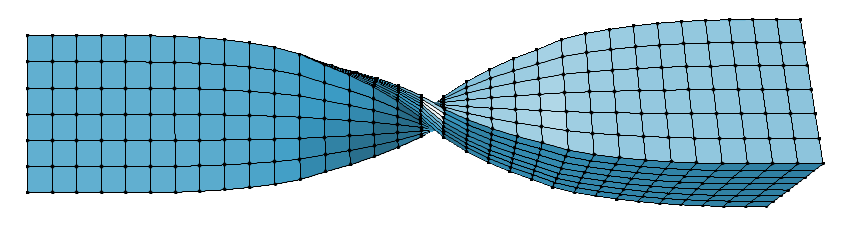
\includegraphics[width=9cm]{01_Skinning/pics/lbsgrad.png}
	\caption[180� Rotation LBS]{ 180� Rotation LBS. Entnommen von \cite{weights}}
	\label{weights_fig1}
\end{figure}

\begin{figure}[t]
	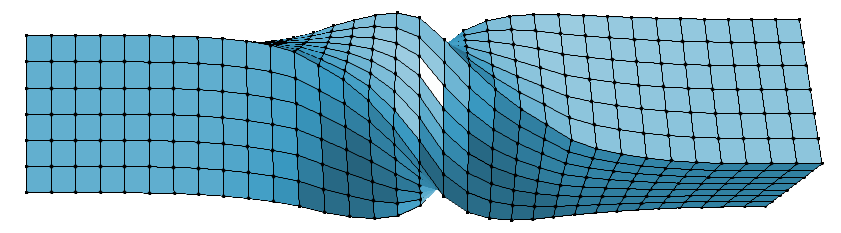
\includegraphics[width=9cm]{01_Skinning/pics/dqsgrad.png}
	\caption[180� Rotation DQS]{180� Rotation DQS. Entnommen von\cite{weights}}
	\label{weights_fig1}
\end{figure}

Die gro�en Vorteile dieser Herangehensweise sind Vermeidung von Artefakten, bei �hnlicher Geschwindigkeit wie beim Linear Blend Skinning. Auch die Implementierung ist unwesentlich schwieriger.

Nachteilhaft ist allerdings das dieser Algorithmus in manchen F�llen mehr Speicher brauchen kann \cite{kavan2008geometric}. Viel schlimmer ist das dieser Algorithmus nur feste Transformationen kann, also zum Beispiel keine Skalierung. \cite{kavan2008geometric} Dies wirkt im ersten Fall nicht schlimm, weil reale Personen kein Volumen verlieren. Im Film ist allerdings durchaus denkbar das ein Charakter sein Volumen, oder die Gr��e einzelner K�rperteile ver�ndern kann. Wodurch bei diesem Ansatz im schlimmsten Fall ein v�llig neues Modell erstellt werden m�sste, wobei es vermutlich einfacher w�re f�r diese Bewegungen einen anderen Algorithmus zu verwenden. Ein weiteres Problem ist das bei Drehungen an einem Gelenk um mehr als 180� das k�rzeste Wege Problem zu Artefakten f�hren kann. \cite{kavan2008geometric} Dargestellt in Abbildung 12. 

\begin{figure}[t]
	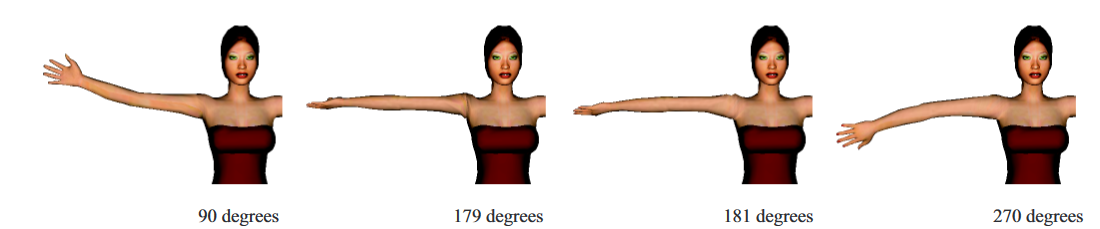
\includegraphics[width=13cm]{01_Skinning/pics/dqsgradartefakte.png}
	\caption[Artefakte DQS bei mehr als 180� Rotation]{Artefakte DQS bei mehr als 180� Rotation Entnommen von \cite{kavan2008geometric}}
	\label{weights_fig1}
\end{figure}
